\section*{Anexo III. Registro de horas}
\label{apendice:clockify}

Este anexo contiene el detalle de todas las entradas registradas en Clockify durante el desarrollo del proyecto.

\subsection*{Descripción}

Clockify es la herramienta de monitorización de tiempo utilizada para registrar todas las horas invertidas en el proyecto. Los registros incluyen:

\begin{itemize}
    \item \textbf{Fecha:} Día de realización de la actividad
    \item \textbf{Duración:} Horas invertidas en la tarea
    \item \textbf{Descripción:} Detalle específico de la actividad realizada
    \item \textbf{Proyecto/Categoría:} Paquete de trabajo de la EDT asociado
    \item \textbf{Tags:} Etiquetas para clasificación (metodología, fase del proyecto)
\end{itemize}

\subsection*{Exportación de datos}


% TODO: Incluir tabla o exportación de Clockify con todos los registros de tiempo

\begin{center}
    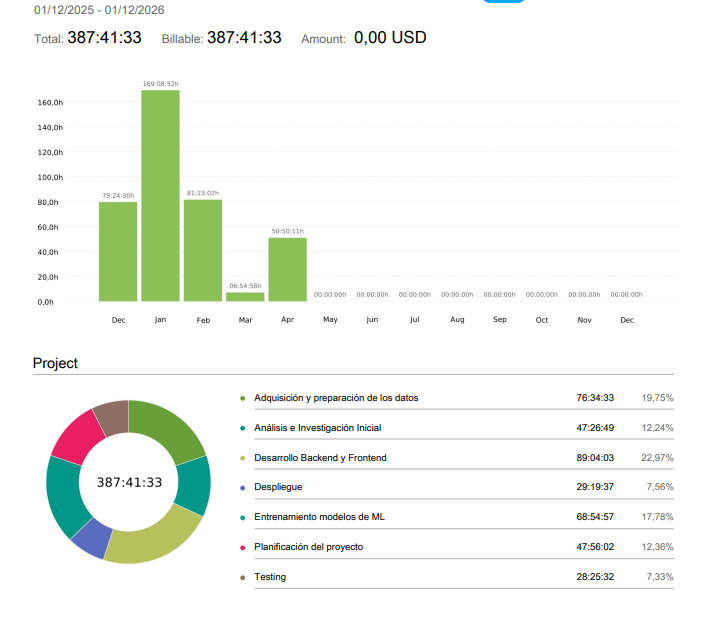
\includegraphics[width=0.5\textwidth]{images/horas.png}
\end{center}

Los registros completos pueden consultarse directamente en la plataforma Clockify en la siguiente URL:

\url{https://app.clockify.me/shared/69ef5bade8cb7f630a26ebc3}
